\documentclass[12pt]{article}
\usepackage[spanish, mexico]{babel}
\usepackage{amsmath}
\usepackage{amsthm}
\usepackage{amssymb}
\usepackage{amsfonts}
\usepackage{IEEEtrantools}
\usepackage{caption}
\usepackage{listings}
\usepackage{graphicx}
\graphicspath{ {images/} }
\pagestyle{headings}
\begin{document}
\title{Apuntes sobre Cálculo Diferencial e Integral III}
\author{Elmer Ortega}
\maketitle
\noindent\section*{Un pequeño recordatorio sobre vectores}
Se conoce a un \textbf{vector} como la conexión de $n$ números 
reales. Se denota como $\vec{v}\in\mathbb{R}^n, \vec{v}=\left(v_1,v_2,v_3\dots,v_n\right)$. 
Además, el conjunto $\mathbb{R}^n$ se define como $\mathbb{R}^n=\left\{a_1,a_2,a_3\dots,a_n | a_i\in\mathbb{R}\right\}$
\newline
\newline
\textbf{Definición de la suma}\newline
Sea $\vec{v}=\left(v_1,v_2,v_3\dots,v_n\right), \vec{u}=\left(u_1,u_2,u_3\dots,u_n\right)$, se define la suma de $\vec{v}+\vec{u}$ como:
\begin{center}
    $\vec{v}+\vec{u}=\left(v_1+u_1,v_2+u_2,\dots,v_i+u_i,\dots,v_n+u_n\right)$
\end{center}
\textbf{Definición del producto por un escalar}\newline
Sea $\lambda\in\mathbb{R},\vec{v}=\left(v_1,v_2,v_3\dots,v_n\right)$, se define el producto de $\lambda*\vec{v}$ como
\begin{center}
    $\lambda*\vec{v}=\left(\lambda v_1, \lambda v_2+,\dots,\lambda v_i,\dots,\lambda v_n\right)$
\end{center}
Todos los $\mathbb{R}^n$ con estas definiciones son un \textbf{espacio vectorial}.
\newline
\textbf{La base canónica en $\mathbb{R}^n$}\newline
Se define a la base canónica de $\mathbb{R}^n$ como el conjunto de:
\begin{center}
    $\vec{e}_1=\left(1,0,0\dots,0\right), \vec{e}_2=\left(0,1,0\dots,0\right), \dots, \vec{e}_n=\left(0,0,0\dots,1\right)$
\end{center}
En especial, la base canónica de $\mathbb{R}^2$ se define como $\left\{i=(1,0),j=(0,1)\right\}$ y $\mathbb{R}^3=\{i=(1,0,0), j=(0,1,0),k=(0,0,1)\}$
Y, ¿por qué es útil? porque puedes pensar los vectores como: 
$\left(a_1,a_2,a_3\dots,a_n\right)=a_1\vec{e}_1+a_2\vec{e}_2+\dots+a_n\vec{e}_n$ 
que es un vector como la combinación lineal de la base canónica y es útil a la hora de diferenciar e integrar.
\newpage
\noindent\textbf{Definición de norma} \newline
Sea el vector $\vec{v}\in\mathbb{R}^n, \vec{v}=(v_1,v_2,\dots,v_n)$, se define la norma de $\vec{v}$ como:\newline
$\|\vec{v}\|=\sqrt{v_1^{2}+v_2^{2}+v_3^{2}+\dots+v_n^2}$, que es igual a la 
\emph{distancia del punto al origen.} \newline
\newline
\textbf{Propiedades de la norma}
\begin{enumerate}
     \item $\|\vec{v}\|\geq0$
     \item $\|\vec{v}\|=0 \Leftrightarrow \vec{v}=\vec{0}$
     \item $\|\lambda\vec{v}\|=|\lambda|\|\vec{v}\|$
     \item Desigualdad del triángulo: $\|\vec{u}+\vec{v}\|\leq \|\vec{u}\|+\|\vec{v}\|$, la igualdad se da 
     $\Leftrightarrow\vec{u}=\lambda\vec{v},\text{ con }\lambda\geq0$
\end{enumerate}

\noindent\textbf{Definición de producto punto o producto interno} \newline
Para  $\vec{u},\vec{v}\in\mathbb{R}^n$, se define el producto punto de $\vec{u}\cdot\vec{v}$ como:
\begin{center}
    $\vec{u}\cdot\vec{v}=u_1v_1+u_2v_2+\dots+u_nv_n$     
\end{center}
\textbf{Propiedades del producto punto}
\begin{enumerate}
     \item $\left(\vec{u}+\vec{v}\right)\cdot\vec{w} = \vec{u}\cdot\vec{w}+\vec{v}\cdot\vec{w}$
     \item $\left(\lambda\vec{u}\right)\cdot\vec{v}=\lambda\left(\vec{u}\cdot\vec{v}\right)$
     \item $\vec{u}\cot\vec{v}=\vec{v}\cot\vec{u}$
     \item $\vec{u}\cdot\vec{u}\geq0$
     \item $\vec{u}\cdot\vec{u}=0\Leftrightarrow\vec{u}=\vec{0}$
     \item $\sqrt{\vec{u}\cdot\vec{u}} = \|\vec{u}\|$
     \item $\cos{\theta}=\dfrac{\vec{u}\cdot\vec{v}}{\|\vec{u}\|}\|\vec{v}\|$, donde $\theta$ es el ángulo
     entre $\vec{u}$ y $\vec{v}$
     \newline
     \textbf{Nota}: $\vec{u}\bot\vec{v}$ (son ortogonales) 
     $\Leftrightarrow$ $\theta=90°=\dfrac{\pi}{2}^r\Leftrightarrow\vec{u}\cdot\vec{v}=0$
\end{enumerate}
\newpage
\noindent\textbf{Representación paramétrica de la recta}
\begin{center}
    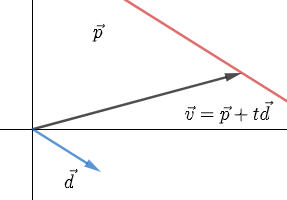
\includegraphics{formaVec.png}
\end{center}
En general, dado $\vec{p}\in\mathbb{R}^n,\vec{d}\in\mathbb{R}^n, \vec{d}\not=\vec{0}, t\in\mathbb{R}$,
\begin{center}
    $\vec{v}=\vec{p}+t\vec{d}$ representa una línea recta en $\mathbb{R}^n$
\end{center}
\textbf{Representación de un hiper-plano}\newline
En general, en $\mathbb{R}^n$, la ecuacion del hiper-plano está dada por,
\begin{center}
    $\left(\vec{v}-\vec{p}\right)\cdot\vec{n}=0$, que es un objeto de dimensión $\mathbb{R}^{n-1}$
\end{center}
Por ejemplo, en $\mathbb{R}^3$, con $\vec{n}=(n_1,n_2,n_3), \vec{p}=(p_1,p_2,p_3), \vec{v}=(x,y,z)$, se tiene que $n_1x+n_2y+n_3z-(n_1p_1+n_2p_2+n_3p_3)=0$, 
por lo que, dado una ecuacion $Ax+By+Cz+F=0$, el vector $\vec{d}=(A,B,C)$ es perpendicular a los vectores $\vec{v}, \vec{p}$


\newpage
\section{Funciones y diferenciación}
\noindent$ \bullet$ Se conoce como funciones con valores escalares o campos escalares a las funciones del tipo $f: \mathbb{R}^n\rightarrow\mathbb{R}$\newline
Por ejemplo, $f: \mathbb{R}^2\rightarrow\mathbb{R}, f(x,y)=3x^2+5xy+e^y$\newline
\newline
$ \bullet$ Se conoce como funciones con valores escalares o campos escalares a las funciones del tipo $f: \mathbb{R}^n\rightarrow\mathbb{R}$\newline
Por ejemplo, $f: \mathbb{R}^2\rightarrow\mathbb{R}, f(x,y)=3x^2+5xy+e^y$\newline
\newline
\textbf{Definición:} Sea $f: \mathbb{R}^n\rightarrow\mathbb{R}$ la \textbf{gráfica} de $f$ es
\begin{center}
    $\left\{(x_1,x_2,x_3,\dots,x_n,f(x_1,x_2,x_3,\dots,x_n)):x_1,x_2,x_3,\dots,x_n\in\mathbb{R}\right\}$
\end{center}
\textbf{Definición:} Se define a las \textbf{curvas de nivel} de $f:\mathbb{R}^2\rightarrow\mathbb{R}$ como
\begin{center}
    $L_c:=\left\{(x,y)\in\mathbb{R}^2: f(x,y)=c\right\}$
\end{center}
\textbf{Definición:} Se define a las \textbf{superficies de nivel} de  $f: \mathbb{R}^3\rightarrow\mathbb{R}$ como
\begin{center}
    $L_c:=\left\{(x,y,z)\in\mathbb{R}^3: f(x,y,z)=c\right\}$
\end{center}
*Notas: La gráfica $f:\mathbb{R}^3\rightarrow\mathbb{R}$ es un objeto que vive en $\mathbb{R}^4$. En general,
 la gráfica $f:\mathbb{R}^n\rightarrow\mathbb{R}$ es un objeto que vive en $\mathbb{R}^{n+1}$.\newline
\textbf{Definición:} Se define al \textbf{conjunto de nivel} de  $f: \mathbb{R}^n\rightarrow\mathbb{R}$ como
 \begin{center}
     $L_c:=\left\{(x_1,x_2,\dots,x_n)\in\mathbb{R}^n: f(x_1,x_2,x_3,\dots,x_n)=c\right\}$
 \end{center}
\subsection*{Conjuntos abiertos y conjuntos cerrados}
\noindent\textbf{Definición:} Dado $\vec{x}_0\in\mathbb{R}^n$ y $\epsilon>0$, la \textbf{bola (abierta)} es el conjunto
 \begin{center}
     $B_{\epsilon}(\vec{x}_0)=\left\{\vec{x}\in\mathbb{R}^n:\|\vec{x}-\vec{x}_0\|<\epsilon\right\}$\newline
     Se le denota como la bola de radio $\epsilon$ centrada en $\vec{x}_0$
 \end{center}
 \textbf{Definición:} Dado un conjunto $A\subseteq\mathbb{R}^n$ es \textbf{abierto} si 
 \begin{center}
     $\forall \vec{x}_0\in A$,existe un $\epsilon > 0 $ tal que $B_\epsilon(\vec{x}_0)\subseteq A$ 
 \end{center}
 \textbf{Proposición:} La bola $B_\epsilon(\vec{x}_0)$ es abierta.\newline
 \textbf{Pd.} $\forall B_\epsilon(\vec{y}_0)\subseteq B_\epsilon(\vec{x}_0)$. Sea $\vec{z}_0\in B_{\epsilon}(\vec{y}_0)$
 \begin{center}
    $\|\vec{z}_0-\vec{x}_0\| = \|\vec{z}_0+\vec{y}_0-\vec{y}_0-\vec{x}_0\|\leq \|\vec{z}_0-\vec{y}_0\|+\|\vec{y}_0-\vec{x}_0\|$ \newline
    $\Rightarrow \|\vec{z}_0-\vec{y}_0\|+\|\vec{z}_0-\vec{x}_0\| < \epsilon - \|\vec{y}_0-\vec{x}_0\|=\epsilon$\newline
    $\Rightarrow \vec{z}_0\in B_{\epsilon}(\vec{x}_0) \therefore \text{ la bola }  B_\epsilon(\vec{x}_0)$ es abierta.
 \end{center}
 \newpage
 \noindent \textbf{Propiedades de los conjuntos abiertos}
\begin{enumerate}
    \item Si $V_1,V_2,V_3,\dots, V_n$  son conjuntos abiertos en $\mathbb{R}^n$, entonces $V_1\cup V_2\cup V_3\cup\dots V_n$ es abierto (Aplica para una union finita e infinita).
    \item Si $V_1,V_2,V_3,\dots, V_n$  son conjuntos abiertos en $\mathbb{R}^n$, entonces $V_1\cap V_2\cap V_3 \cap \dots V_n$ es abierto (Solo para una intersección finita).
    \item $\mathbb{R}^n$ es abierto.
    \item $\emptyset$ es abierto. $\rightarrow$ argumento de vacuidad o vacío.
\end{enumerate}
\noindent\subsection*{Puntos frontera}
\noindent \textbf{Definición: } Sea $A \in \mathbb{R}_n$. Un punto $\vec{x}_0 \in \mathbb{R}^n$ es un \textbf{punto frontera}
de $A$ si todas las bolas abiertas centradas en $\vec{x}_0$ tienen en $A$ y puntos no en $A$. \newline \newline
El conjunto de puntos frontera de $A$ se llama la \textbf{frontera de } $A$.\newline
\textbf{Ejemplos de puntos fronteras:}

\begin{center}
    \begin{tabular}{| c | c |}
    \hline
    Conjunto $A$ & frontera de $A$ \\
    \hline
    $A=(-2,3)\subseteq\mathbb{R}$ & $\{-2,3\}$  \\
    $A=[-2,3)\subseteq\mathbb{R}$ & $\{-2,3\}$  \\
    $A=(-2,3)\cup\{ 6 \}\subseteq\mathbb{R}$ & $\{-2,3,6\}$  \\
    $A=(-2,3)\cup[3,6)\subseteq\mathbb{R}$ & $\{-2,6\}$  \\
    $A=(-2,3)\cup(3,6]\subseteq\mathbb{R}$ & $\{-2,3,6\}$  \\
    $A=\{x\in\mathbb{Q} : 0\leq x \leq 1\}$ & $[0,1]$ \\
    $A=\{(x,y)\in\mathbb{R}^2:x^2+y^2<1\}$ & $\{(x,y)\in\mathbb{R}^2:x^2+y^2=1\}$ \\
    $A$ es un finito& El mismo conjunto $A$\\
    $A=\left\{1+\dfrac{1}{n}:n\in\mathbb{N}\right\}=\left\{2,1+\dfrac{1}{2},\dots\right\}$ & $A\cup \{1\}$\\
    $A=\mathbb{R}^n$ & $\emptyset$\\
    $A=\emptyset$ & $\emptyset$\\
    \hline
    \end{tabular}
    \end{center}
\newpage
\noindent \textbf{Definición: }  Sea $B\subseteq\mathbb{R}^n$. Decimos que $B$ es un conjunto \textbf{cerrado} si $B^c$ es \emph{abierto}.
\newline\newline
\textbf{Propiedades de conjuntos cerrados: }
\begin{enumerate}
    \item Si $V_1,V_2,V_3,\dots, V_n$  son conjuntos cerrados en $\mathbb{R}^n$, entonces $V_1\cup V_2\cup V_3\cup\dots V_n$ es abierto (Solo para una intersección finita).
    \item Si $V_1,V_2,V_3,\dots, V_n$  son conjuntos abiertos en $\mathbb{R}^n$, entonces $V_1\cap V_2\cap V_3 \cap \dots V_n$ es abierto (Aplica para una union finita e infinita).
    \item $\emptyset$ es cerrado.
    \item$\mathbb{R}^n$ es cerrado.
\end{enumerate}
\noindent\textbf{*Nota: }$\empty$ y $\mathbb{R}^n$ son los únicos conjuntos abiertos y cerrados.\newline
\noindent\textbf{*Nota: }La frontera de $A$ y $A^c$ es el mismo conjunto. \newline
\noindent\textbf{*Nota: }Si $A$ es un conjunto finito de $\mathbb{R}^n$, entoces $A$ es cerrado y no abierto.\newline
\noindent\textbf{*Nota:}\"{}Entre 2 números racionales, hay un irracional y hay un racional entre 2 números irracionales\"{}.\newline
\begin{center}
    \begin{tabular}{| c | c |}
    \hline
    Conjunto $A$ & Características de $A$ \\
    \hline
    $A=\{(x,y)\subseteq\mathbb{R}^2:y\leq x^2\}$ & Pensando en $y=x^2\rightarrow A^c$ es abierto $\therefore A$ es cerrrado  \\
    $A={(1,1,1)}\subseteq\mathbb{R}^3$ & $A$ es cerrado  \\
    $A=[2,5]\subseteq\mathbb{R}$ & Como $A^c=(-\infty,2)\cup(5\,\infty)$ es abierto $\therefore A$ es cerrado  \\
    $A=[2,5)\subseteq\mathbb{R}$ & A  es no abierto y no cerrado   \\
    $A=[2,\infty)\subseteq\mathbb{R}$ & Como $A^c=(-\infty,2)$ es abierto, A es cerrado  \\
    $A=\{x\in\mathbb{Q} : 0\leq x \leq 1\}$ & $A$ es no abierto, no cerrado\\
    $A=\left\{1+\dfrac{1}{n}:n\in\mathbb{N}\right\}$ & $A$ es no abierto, no cerrado \\
    \hline
    \end{tabular}
    \end{center}
\newpage
\section*{Límites}
\noindent\textbf{Definición de límite:} Sea $f:A\subseteq\mathbb{R}^n\rightarrow\mathbb{R}^m$ con $A$ abierto y 
sea $\vec{a}\in A$\newline
Decimos que
\begin{center}
    $\lim_{\vec{x}\rightarrow\vec{a}}{f(\vec{x})} = \vec{b}$ , $(\vec{b}\in\mathbb{R}^m)$ 
\end{center}
\noindent Si $\forall \epsilon>0, \exists \delta >0 $ tq si $\vec{x}\in A$ y $\|\vec{x}-\vec{a}\| < \delta \Rightarrow  \|f(\vec{x})-\vec{b}\| < \epsilon$.\newline
Para mostrar que un límite no existe es necesario mostrar dos trayectorias (ecuaciones) tales que el limite sea diferente en ellas.
\newline
\newline
\textbf{Propiedades de los límites: }\newline
\noindent Sea $f\subseteq\mathbb{R}^n\rightarrow\mathbb{R}^m, g\subseteq\mathbb{R}^n\rightarrow\mathbb{R}^m$ y sea $\vec{a}\in A$ o en la frontera de $A$.
\begin{enumerate}
    \item Si $\lim_{\vec{x}\rightarrow\vec{a}}{f(\vec{x})}=\vec{L}$ y $\lim_{\vec{x}\rightarrow\vec{a}}{g(\vec{x})}=\vec{M}$\newline
            $\Rightarrow\lim_{\vec{x}\rightarrow\vec{a}}{f(\vec{x})+g(\vec{x})}=\vec{L}+\vec{M}$
    \item Si $c\in\mathbb{R}$ y $\lim_{\vec{x}\rightarrow\vec{a}}{f(\vec{x})}=\vec{L}$\newline
            $\Rightarrow\lim_{\vec{x}\rightarrow\vec{a}}{cf(\vec{x})}=c\vec{L}$
    \item Si $m=1$ (Imagen), $\lim_{\vec{x}\rightarrow\vec{a}}{f(\vec{x})}=\vec{L}$ y $\lim_{\vec{x}\rightarrow\vec{a}}{g(\vec{x})}=\vec{M}$\newline
            $\Rightarrow\lim_{\vec{x}\rightarrow\vec{a}}{f(\vec{x})g(\vec{x})}=L*M$
    \item Si $m=1$ (Imagen), $\lim_{\vec{x}\rightarrow\vec{a}}{f(\vec{x})}=\vec{L} \not=0$\newline
            $\Rightarrow\lim_{\vec{x}\rightarrow\vec{a}}{ \dfrac{1}{f(\vec{x})} }=\dfrac{1}{L}$
    \item Si $m>1$ y $f(\vec{x})=\left( f_1(\vec{x}),f_2(\vec{x}), \dots, f_m(\vec{x})\right)\text{ con } f_i:A\subseteq\mathbb{R}^n\rightarrow\mathbb{R}^m$\newline
            $\Rightarrow \lim_{\vec{x}\rightarrow\vec{a}}{f(\vec{x})}=\vec{L}\Leftrightarrow\lim_{\vec{x}\rightarrow\vec{a}}{f_i(\vec{x})}=\vec{L_i}, \forall i=1,2,3,\dots,m$ donde $\vec{L}=(L_1,L_2,L_3,\dots, L_m)$
\end{enumerate}
\newpage
\subsection*{Continuidad}
\textbf{Definición:} Sea $f:A\subseteq\mathbb{R}^n\rightarrow\mathbb{R}^m y sea \vec{a}\in A.$ Decimos que $f$ es \emph{continua} en
$\vec{a}$ si
\begin{center}
    $\lim_{\vec{x}\rightarrow\vec{a}}{f(\vec{x})}=f(\vec{a})$
\end{center}
\textbf{Propiedades de continuidad puntual: }\newline
\noindent Sea $f\subseteq\mathbb{R}^n\rightarrow\mathbb{R}^m, g\subseteq\mathbb{R}^n\rightarrow\mathbb{R}^m$ y sea $\vec{a}\in A$ y $c\in\mathbb{R}$.
\begin{enumerate}
    \item Si $f$ y $g$ son \emph{continuas en } $\vec{a}$
            \begin{center}
                $\Rightarrow f+g$ es \emph{continua en} $\vec{a}$
            \end{center}
    \item Si $f$ es \emph{continua en } $\vec{a}$
            \begin{center}
                $\Rightarrow cf$ es \emph{continua en} $\vec{a}$ 
            \end{center}
    \item Si $m=1$ (Imagen), $f$ y $g$ son \emph{continuas en } $\vec{a}$
            \begin{center}
                $\Rightarrow f\cdot{}g$ es \emph{continua en } $\vec{a}$
            \end{center}
    \item Si $m=1$ (Imagen), $f$ es \emph{continua en } $\vec{a}$ y $f(\vec{a})\not = 0$
            \begin{center}
                $\Rightarrow \dfrac{1}{f}$ es \emph{continua en } $\vec{a}$
            \end{center}
    \item Si $m>1$ y $f(\vec{x})=\left(f_1(\vec{x}),f_2(\vec{x}),\dots,f_m(\vec{x})\right)$
            \begin{center}
                $\Rightarrow f$ es \emph{continua en} $\vec{a} \Leftrightarrow f_i$ es \emph{continua en} $\vec{a}$ ,$\forall i=1,2,\dots,m$
            \end{center}
\end{enumerate}

\noindent\textbf{Definición (semi-formal):} Sea $f:\mathbb{R}^n\rightarrow\mathbb{R}^m$, se dice que $f$ es un \emph{polinomio} si es una
combinación lineal de productos de potencias no negativas de $x_i\in\mathbb{R}^n$ con $i=1,2,3\dots,n$.\newline

\noindent\textbf{Teorema (semi-formal):} Si $f(\vec{x})$ es un polinomio entonces $f$ es \emph{continua } para todo $\vec{a}$.\newline
\newline
\noindent\textbf{Teorema (semi-formal):} Si $f(\vec{x})$ es una \emph{función racional}, es decir, cociente de polinomios
entonces $f$ es \emph{continua en} $\vec{a}$ si el denominador de $f(\vec{x})\not=0$ en $\vec{a}$.\newline
\newline
\newpage
\noindent\textbf{Composición de funciones}\newline
\textbf{Teorema: }Si $g:A\subseteq\mathbb{R}^n\rightarrow \mathbb{R}^m$ y $f:b\subseteq\mathbb{R}^m\rightarrow \mathbb{R}^p$ y 
$f(A)\subseteq B$ y $f$ es continua en $\vec{a}$ y$g$ es continua en $f(\vec{a})\Longrightarrow$ 
\begin{center}
    $g\circ f$ es \emph{continua} en $\vec{a}$
\end{center}
\noindent \textbf{Observación} Una funcion $f$ es \emph{continua} en un conjunto $A$ si es continua en cada vector $\vec{a}$.
\newpage
\subsection*{Derivadas}
\noindent \textbf{Definición:} Se define como \emph{derivada parcial de $f$ con respecto a $x$ en $(a,b)$}
\begin{center}
    $\dfrac{\partial f}{\partial x}{(a,b)}:=\lim_{h\rightarrow0}{\dfrac{f(a+h,b)-f(a,b)}{h}}$
\end{center}
\noindent \textbf{Definición:} Se define como \emph{derivada parcial de $f$ con respecto a $y$ en $(a,b)$}
\begin{center}
    $\dfrac{\partial f}{\partial y}{(a,b)}:=\lim_{k\rightarrow0}{\dfrac{f(a,b+k)-f(a,b)}{k}}$
\end{center}
\noindent En general, sea $f:u\subseteq\mathbb{R}^n\rightarrow \mathbb{R}$ con $u$ abierto, 
se define a la \emph{derivada parcial en dirección de $x_i$}: 
\begin{center}
    $\dfrac{\partial f}{\partial x_i}{(a_1,a_2,\dots,a_n)}:=\lim_{h\rightarrow0}{\dfrac{f(a_1,a_2,\dots,x_i+h ,\dots,a_n)-f(a_1,a_2,\dots,a_n)}{h}}$
    \indent $=\lim_{h\rightarrow0}{\dfrac{f(\vec{a}+h\vec{e_i})-f(\vec{a})}{h}}$
\end{center}
\noindent \textbf{Notación: }
\begin{center}
    $\dfrac{\partial f}{\partial x_i}$, $\dfrac{\partial f}{\partial x_i}|_{\vec{x}=\vec{a}}$, $f_{(x_i)}(\vec{a})$, $D_{x_i}f(\vec{a})$
\end{center}
\noindent La \textbf{ecuación del plano tangente} a la superficie $z=f(x,y)$ está dada por la ecuación:
\begin{center}
    $z=\dfrac{\partial f(x_0,y_0)}{\partial x}(x-x_0)+\dfrac{\partial f(x_0,y_0)}{\partial y}(y-y_0)+f(x_0,y_0)$
\end{center}
\noindent \textbf{Definición:} Sea $U\subseteq\mathbb{R}^2$ abierto y $f:U\rightarrow\mathbb{R}$. Decimos que $f$ es 
\textbf{diferenciable} en $(x_0,y_0)\in U$ si $\dfrac{\partial f(x_0,y_0)}{\partial x}$ y $\dfrac{\partial f(x_0,y_0)}{\partial y}$
existen y 

    ${\lim_{(x,y)\rightarrow(x_0,y_0)}{\dfrac{f(x,y)-f(x_0,y_0)-\dfrac{\partial f(x_0,y_0)}{\partial x}{(x-x_0)}-\dfrac{\partial f(x_0,y_0)}{\partial y}{(y-y_0)}}{\|(x,y)-(x_0,y_0)\|}}=0}$


\noindent Solamente diremos que \textbf{existe} el plano tangente en $(x_0,y_0)$ si $f$ es diferenciable en $(x_0,y_0)$
\newline
\newpage
\noindent \textbf{Definición:} El \textbf{gradiente de }$f$ es el vector
\begin{center}
    $\nabla f(x_0,y_0)=\left(\dfrac{\partial f(x_0,y_0)}{\partial x},\dfrac{\partial f(x_0,y_0)}{\partial y} \right)$
\end{center}
\noindent También se denota como $Df(x_0,y_0)$ o $(grad\text{ }f)(x_0,y_0)$

Entonces la definición de \textbf{diferenciabilidad} se puede leer como el gradiente existe:
\begin{center}
    ${\lim_{(x,y)\rightarrow(x_0,y_0)}{\dfrac{f(x,y)-f(x_0,y_0)-\left(\nabla f(x_0,y_0)\right)\cdot\left(x-x_0,y-y_0\right)}{\|(x,y)-(x_0,y_0)\|}}=0}$
\end{center}

\noindent \textbf{Definición: }El gradiente de una función $f\subseteq\mathbb{R}^n\rightarrow\mathbb{R}$, con $A$ abierto, es:
\begin{center}
    $\nabla{f(\vec{x_0})}:=\left(\dfrac{\partial f(x_0,y_0)}{\partial x_1},\dfrac{\partial f(x_0,y_0)}{\partial x_2},\dots,\dfrac{\partial f(x_0,y_0)}{\partial x_n}\right)$
\end{center}

\noindent \textbf{Definición: } Sea $f\subseteq\mathbb{R}^n\rightarrow\mathbb{R}$. Decimos que $f$ es \emph{diferenciable} en un 
punto $\vec{x_0}\in A$ si $\dfrac{\partial f}{\partial x_i}(\vec{x_0})$ existen $\forall i=1,2,\dots,n$ y 
\begin{center}
    ${\lim_{(\vec{x})\rightarrow(\vec{x_0})}{\dfrac{f(\vec{x})-f(\vec{x_0})-\left(\nabla f(\vec{x_0})\right)\cdot\left(\vec{x}-\vec{x_0}\right)}{\|\vec{x}-\vec{x_0}\|}}=0}$
\end{center}
\noindent Mientras mas cerca este $\vec{x}$ de $\vec{x_0}$ mejor será la aproximación, ya que, el límite indica que la diferencia entre
el plano y la gráfica es mejor que la diferencia entre $\vec{x}$ y $\vec{x_0}$. Entonces, solo y solo en este caso decimos que $T(\vec{x})= f(\vec{x_0})+\left(\nabla f(\vec{x_0})\right)\cdot\left(\vec{x}-\vec{x_0}\right)$
es el plano tangente de $\vec{x_0}$. Así, aunque las  $\dfrac{\partial{f}}{\partial{x_i}}{(\vec{x_0})}$ existan es solo una razón necesaria más no suficiente.

\newpage
\noindent \textbf{Definición: } Sea $f:A\subseteq\mathbb{R}^n\rightarrow\mathbb{R}^m$ y $\vec{x_0}\in A$ con $A$ abierto. 
Supongamos que $f(f_1,f_2, \dots, f_m)$. Si $\dfrac{\partial{f_i}}{\partial{x_j}}{(\vec{x_0})}$ existe, denotamos
\begin{center}
    \begin{equation}\notag
        Df(\vec{x_0})=
        \begin{pmatrix}
        \dfrac{\partial{f_1}}{\partial{x_1}}{(\vec{x_0})} & \dfrac{\partial{f_1}}{\partial{x_2}}{(\vec{x_0})}& \cdots & \dfrac{\partial{f_1}}{\partial{x_n}}{(\vec{x_0})}\\
        \dfrac{\partial{f_2}}{\partial{x_1}}{(\vec{x_0})} & \dfrac{\partial{f_2}}{\partial{x_2}}{(\vec{x_0})} & \cdots & \dfrac{\partial{f_2}}{\partial{x_n}}{(\vec{x_0})}\\
        \vdots & \vdots & \ddots & \vdots\\
        \dfrac{\partial{f_m}}{\partial{x_1}}{(\vec{x_0})} & \dfrac{\partial{f_m}}{\partial{x_2}}{(\vec{x_0})}& \cdots & \dfrac{\partial{f_m}}{\partial{x_n}}{(\vec{x_0})}
        \end{pmatrix}
        \end{equation}
\end{center}
\noindent A esta matriz se conoce como la \textbf{matriz jacobiana de $f$ (en $\vec{x_0}$)} y es de tamaño $m\times n$

\noindent \textbf{Definición: }Sea $f:A\subseteq\mathbb{R}^n\rightarrow\mathbb{R}^m$ y $\vec{x_0}\in A$ con $A$ abierto. Decimos que 
$f$ es \emph{diferenciable en} $\vec{x_0}$ si $\dfrac{\partial{f_i}}{\partial{x_m}}{(\vec{x_0})}$ existen $\forall i,j$ y 
\begin{center}
    ${\lim_{(\vec{x})\rightarrow(\vec{x_0})}{\dfrac{f(\vec{x})-f(\vec{x_0})-\left(Df(\vec{x_0})\right)\cdot\left(\vec{x}-\vec{x_0}\right)}{\|\vec{x}-\vec{x_0}\|}}=0}$
\end{center}
\noindent Si el $lim\not=0$ $T(\vec{x_0})=f(\vec{x_0})+ Df(\vec{x_0})\cdot (\vec{x}-\vec{x_0})$ no se interpreta como un plano tangente.

\noindent \textbf{Teorema: }Sea $f:A\subseteq\mathbb{R}^n\rightarrow\mathbb{R}^m$ y $\vec{x_0}\in A$ con $A$ abierto. Si $f$ es diferenciable en $\vec{x_0}$, entonces
\begin{center}
    $f$ es continua en $\vec{x_0}$
\end{center}

\noindent \textbf{Nota: }Es posible que las derivadas parciales existan pero la función no sea continua.

\noindent \textbf{Teorema: }Sea $f:A\subseteq\mathbb{R}^n\rightarrow\mathbb{R}^m$ y $\vec{x_0}\in A$ con $A$ abierto. Si $f$ es diferenciable en $\vec{x_0}$, supongamos que 
$\dfrac{\partial{f_i}}{\partial{x_j}}$ existe y es continua en $B_{r}(\vec{x_0})$, para algun $r>0$ y $\forall i,j$, entonces $f$ es \emph{diferenciable en} $\vec{x_0}$

\noindent \textbf{Notación: }Sea $f:A\subseteq\mathbb{R}^n\rightarrow\mathbb{R}^m$ con $A$ abierto, decimos que $f$ es de clase $C^{1}$ en $A$ si $\dfrac{\partial{f_i}}{\partial{x_j}}$ existen y son continuas en $A$.\newline

\subsection*{Trayectorias} 

\noindent \textbf{Definción: }Una función $f:I\subseteq\mathbb{R}\rightarrow \mathbb{R}^n$ (usualmente  $f$ es continua) es un \textbf{trayectoria}. Usualmente, a los compenentes de $f$ las llamamos
$X_i(t)$; i,e,
\begin{center}
    $f(t)=(X_1 (t),X_2 (t),\dots,X_n (t))$
\end{center}
\noindent donde $t$ se le conoce como parametro y la imagen de $f$ le llamamos la curva. 

\noindent Pensando en la curva de f, tendremos un vector $c'(t_0)$ que es el vector de velocidad instantánea. Y
$\|c'(t_0)\|$ es la rapidez de la curva en $t_0$

\noindent \textbf{Definición:} Si $C:\mathbb{R}\rightarrow\mathbb{R}^n$ es una trayectoria y $c'(t_0)$ existe, entonces
\begin{center}
    $U(t)=c(t_0)+tc'(t_0)$
\end{center}
es la ecuacion de la recta con posición inicial $c(t_0)$ y vector de dirección $c'(t_0)$

\subsection*{Proposiciones de derivadas} 
\noindent \textbf{Proposición:} Sea $f:A\subseteq\mathbb{R}^n\rightarrow\mathbb{R}^m$ con $A$ abierto y $\vec{x_0}\in A$. Si $f$ es diferenciable en 
$\vec{x_0}$ y $c\in\mathbb{R}$ entonces $cf$ es diferenciable en $\vec{x_0}$ y 
\begin{center}
    $D(cf)(\vec{x_0})=cD(f)(\vec{x_0})$
\end{center}

\noindent \textbf{Proposición:} Sean $f,g:A\subseteq\mathbb{R}^n\rightarrow\mathbb{R}^m$ con $A$ abierto y $\vec{x_0}\in A$. Si $f$ y $g$ son diferenciable en 
$\vec{x_0}$ entonces $f+g$ es diferenciable en $\vec{x_0}$ y 
\begin{center}
    $D(f+g)(\vec{x_0})=Df(\vec{x_0})+Dg(\vec{x_0})$
\end{center}

\noindent \textbf{Proposición: }Además, si $m=1$, $f\circ g$ es diferenciable en $\vec{x_0}$, y 
\begin{center}
    $D(f\cdot g)(\vec{x_0})=f(\vec{x_0})Dg(\vec{x_0})+g(\vec{x_0})Df(\vec{x_0})$
\end{center}

\noindent \textbf{Proposición:} Sean $f,g:A\subseteq\mathbb{R}^n\rightarrow\mathbb{R}$ con $A$ abierto y $\vec{x_0}\in A$. Si $f$ y $g\not=0$ son diferenciable en 
$\vec{x_0}$ entonces $\dfrac{f}{g}$ es diferenciable en $\vec{x_0}$ y 
\begin{center}
    $D(\dfrac{f}{g})(\vec{x_0})=\dfrac{g(\vec{x_0})Df(\vec{x_0})-f(\vec{x_0})Dg(\vec{x_0})}{(g{\vec{x_0}})^2}$
\end{center}

\noindent \textbf{Teorema (Regla de la cadena):} Sean $g:\subseteq\mathbb{R}^n\rightarrow\mathbb{R}^m$ y $f:\subseteq\mathbb{R}^m\rightarrow\mathbb{R}^p$.
Si $g$ es diferenciable en $\vec{x_0}\in \mathbb{R}^n$ y $f$ es diferenciable en $g(\vec{x_0})$ y entonces
$f\circ g:\mathbb{R}^n\rightarrow\mathbb{R}^p$ es diferenciable en $\vec{x_0}$ y
\begin{center}
    $D(f\circ g)(\vec{x_0})=Df(g(\vec{x_0}))Dg(\vec{x_0})$
\end{center}




\end{document}
